\documentclass[18pt]{beamer}

\title[Reordering in Statistical Machine Translation for Chinese]{Analyzing the Potential of Source Sentence Reordering in Statistical Machine Translation}
\author{Ge Wu}

% Bibliography
\usepackage{xcolor}
\usepackage{tabu}
\usepackage{tikz}
\usepackage{CJK}
\usetikzlibrary{arrows,positioning} 
\usepackage[citestyle=authoryear,bibstyle=numeric,hyperref,backend=biber]{biblatex}

\addbibresource{templates/example.bib}
\bibhang1em

\begin{document}

%title page
\begin{frame}
\titlepage
\end{frame}

\begin{frame}{Illustration}
\begin{tabu}{ll}
English & The black cat climbed to the tree top.\\
\rowfont{\color{blue}} Spanish & The cat black climbed to the top tree.\\
\rowfont{\color{red}} Japanese & The black cat the tree top to climbed.\\
\end{tabu}
\end{frame}

\begin{frame}{Illustration}
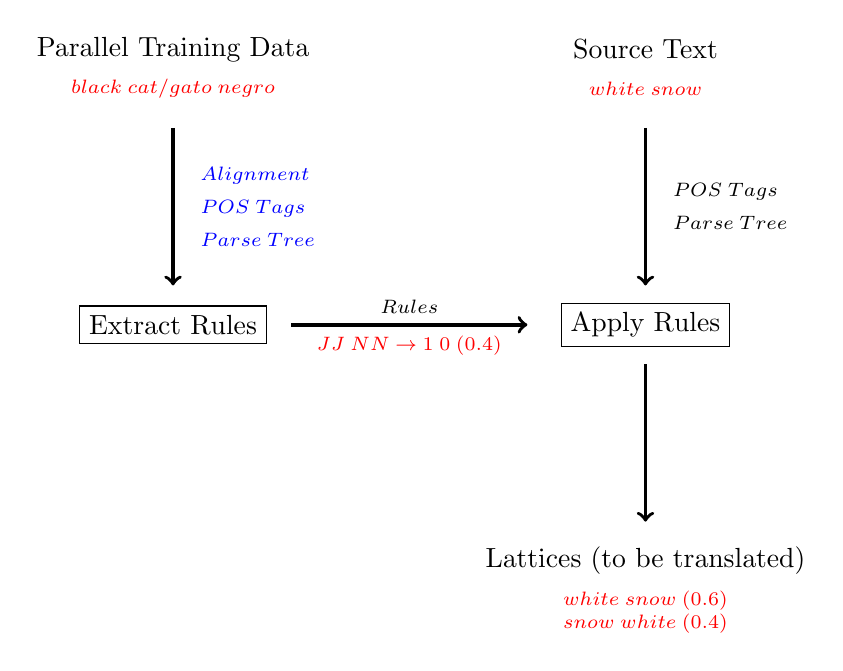
\begin{tikzpicture}
\tikzstyle{myarrows}=[->,line width=0.45mm];
\node[rectangle](x1) at (0,0.5){Parallel Training Data};
\node[rectangle] at(0, 0) {\textcolor{red}{$\scriptstyle black \hspace{0.2em}cat / gato \hspace{0.2em}negro$}};
\node[rectangle,draw](x2) at (0,-3){Extract Rules};
\node[rectangle](x3) at (6,0.5){Source Text};
\node[rectangle] at(6, 0) {\textcolor{red}{$\scriptstyle white \hspace{0.2em}snow$}};
\node[rectangle,draw](x4) at (6,-3){Apply Rules};
\node[rectangle](x5) at (6,-6){Lattices (to be translated)};
\node[rectangle] at(6, -6.5) {\textcolor{red}{$\scriptstyle white \hspace{0.2em}snow\hspace{0.2em}(0.6)$}};
\node[rectangle] at(6, -6.8) {\textcolor{red}{$\scriptstyle snow \hspace{0.2em}white\hspace{0.2em}(0.4)$}};
\draw [myarrows] (0,-0.5) -- node[auto] {\begin{tabular}{l}
    \color{blue}{$\scriptstyle Alignment$} \\
    \color{blue}{$\scriptstyle POS\hspace{0.2em}Tags$}\\ 
    \color{blue}{$\scriptstyle Parse\hspace{0.2em}Tree$}
\end{tabular}} (0,-2.5);
\draw [myarrows] (6,-0.5) -- node[auto] {\begin{tabular}{l}
    \color{black}{$\scriptstyle POS\hspace{0.2em}Tags$}\\ 
    \color{black}{$\scriptstyle Parse\hspace{0.2em}Tree$}
\end{tabular}} (6,-2.5);
\draw [myarrows] (6,-3.5) -- (6,-5.5);
\draw [myarrows] (1.5,-3) -- node[auto] {$\scriptstyle Rules$}  node[below] {\textcolor{red}{$\scriptstyle JJ\hspace{0.2em} NN \hspace{0.2em}\rightarrow\hspace{0.2em} 1\hspace{0.2em} 0 \hspace{0.2em}(0.4)$}} (4.5,-3);
\end{tikzpicture}
\end{frame}

\begin{frame}[fragile]{Alignment}
\verb|1  2  3   4 5 6   7   8      9    10 11 12| \\
On the 24th , a series of attacks occurred in Iraq .\\
%\vspace{1cm}

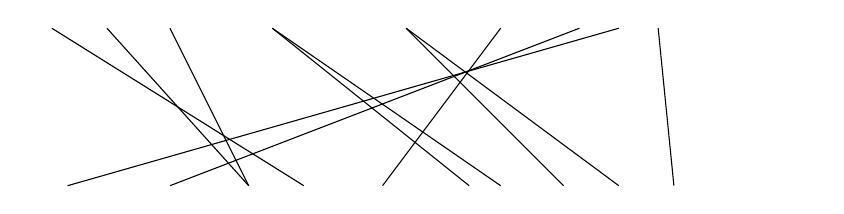
\begin{tikzpicture}
\draw [white] (0,0) rectangle (10,2);
\draw (0.5,0) -- (7.5,2);
\draw (1.8,0) -- (7,2);
\draw (2.8,0) -- (1.8,2);
\draw (3.5,0) -- (0.3,2);
\draw (2.8,0) -- (1,2);
\draw (4.5,0) -- (6,2);
\draw (6,0) -- (3.1,2);
\draw (5.6,0) -- (3.1,2);
\draw (6.8,0) -- (4.8,2);
\draw (7.5,0) -- (4.8,2);
\draw (8.2,0) -- (8,2);
\end{tikzpicture}
\begin{CJK}{UTF8}{gbsn} \\
伊拉克 境内 二十四 号 发生 了 多 起 袭击 事件 。
\end{CJK}
\verb|   1    2    3    4  5  6  7  8  9   10 11| \\
\vspace{1cm}
1-4 2-3 3-3 6-7 6-8 8-9 8-10 9-5 10-2 11-1 12-11
\end{frame}

\begin{frame}[fragile]{POS Tags}
On the 24th , a series of attacks occurred in Iraq .\\
\vspace{0.5cm}
\verb|IN DT  JJ , DT NN IN  NNS    VVN IN NP SENT| \\
\end{frame}

\begin{frame}{Parse Tree}
\begin{figure}
\centering
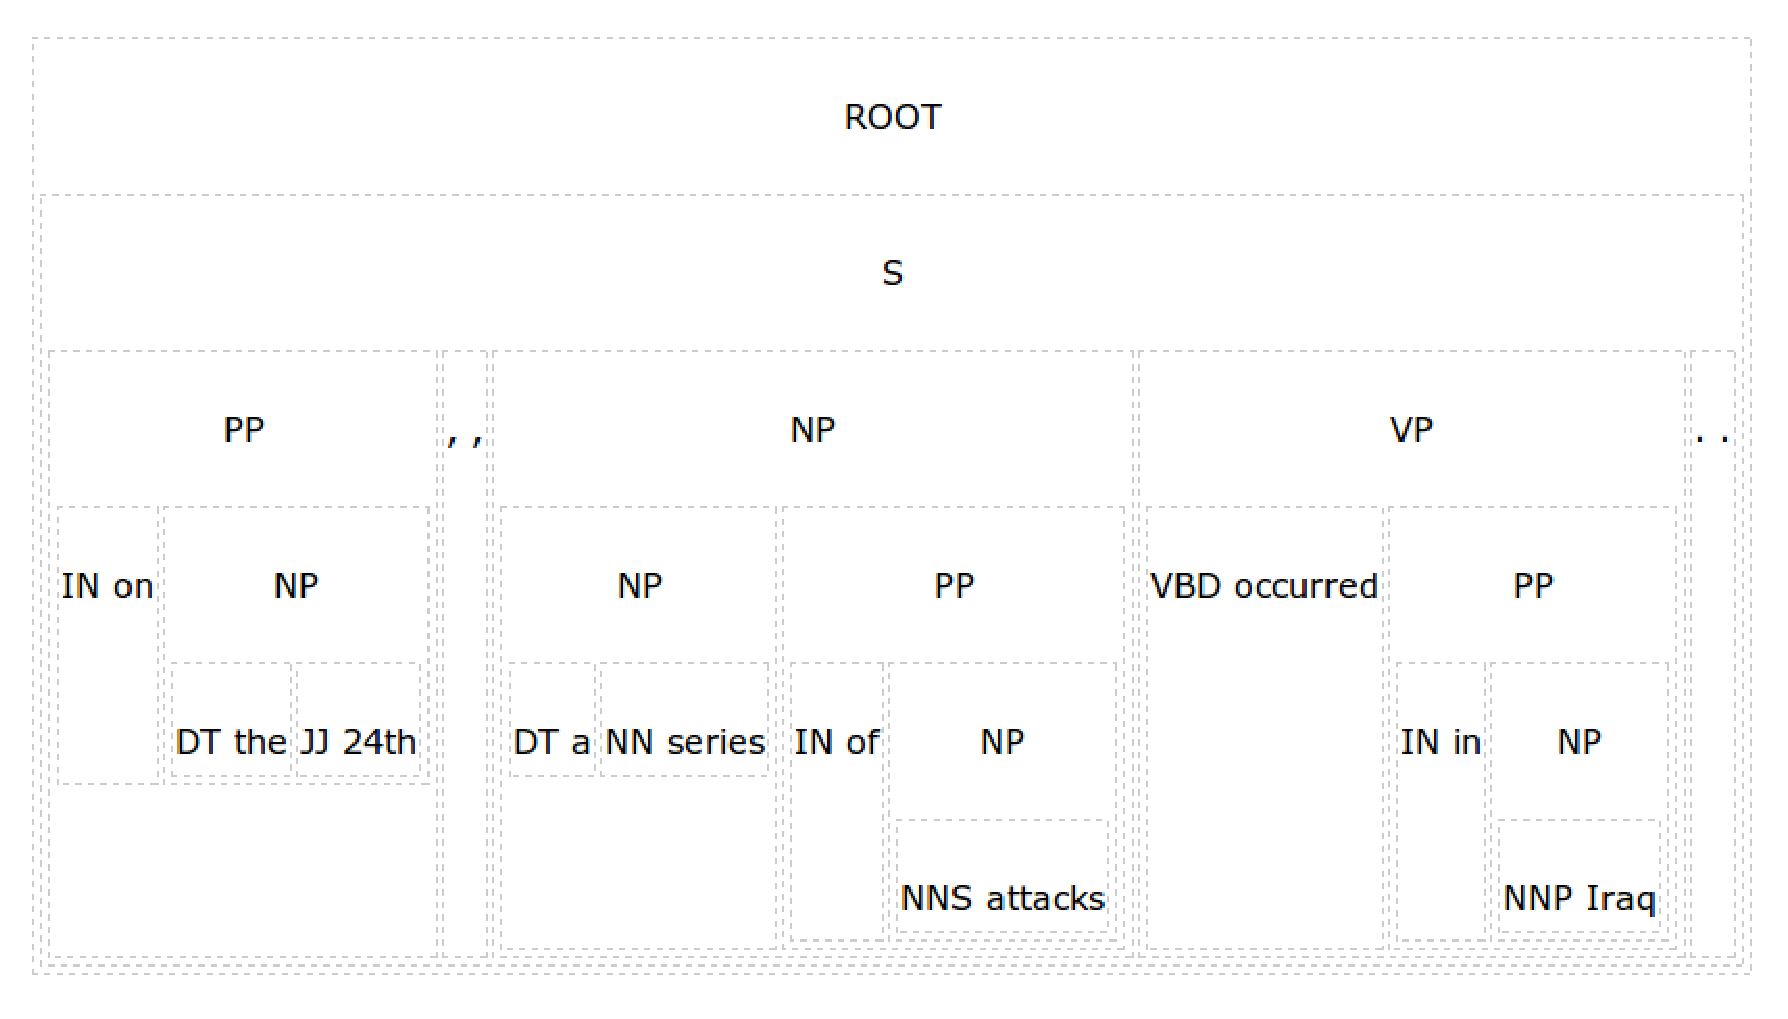
\includegraphics[scale=0.36]{tree.eps}
\end{figure}
\end{frame}

\begin{frame}{Lattices}
\begin{figure}
\centering
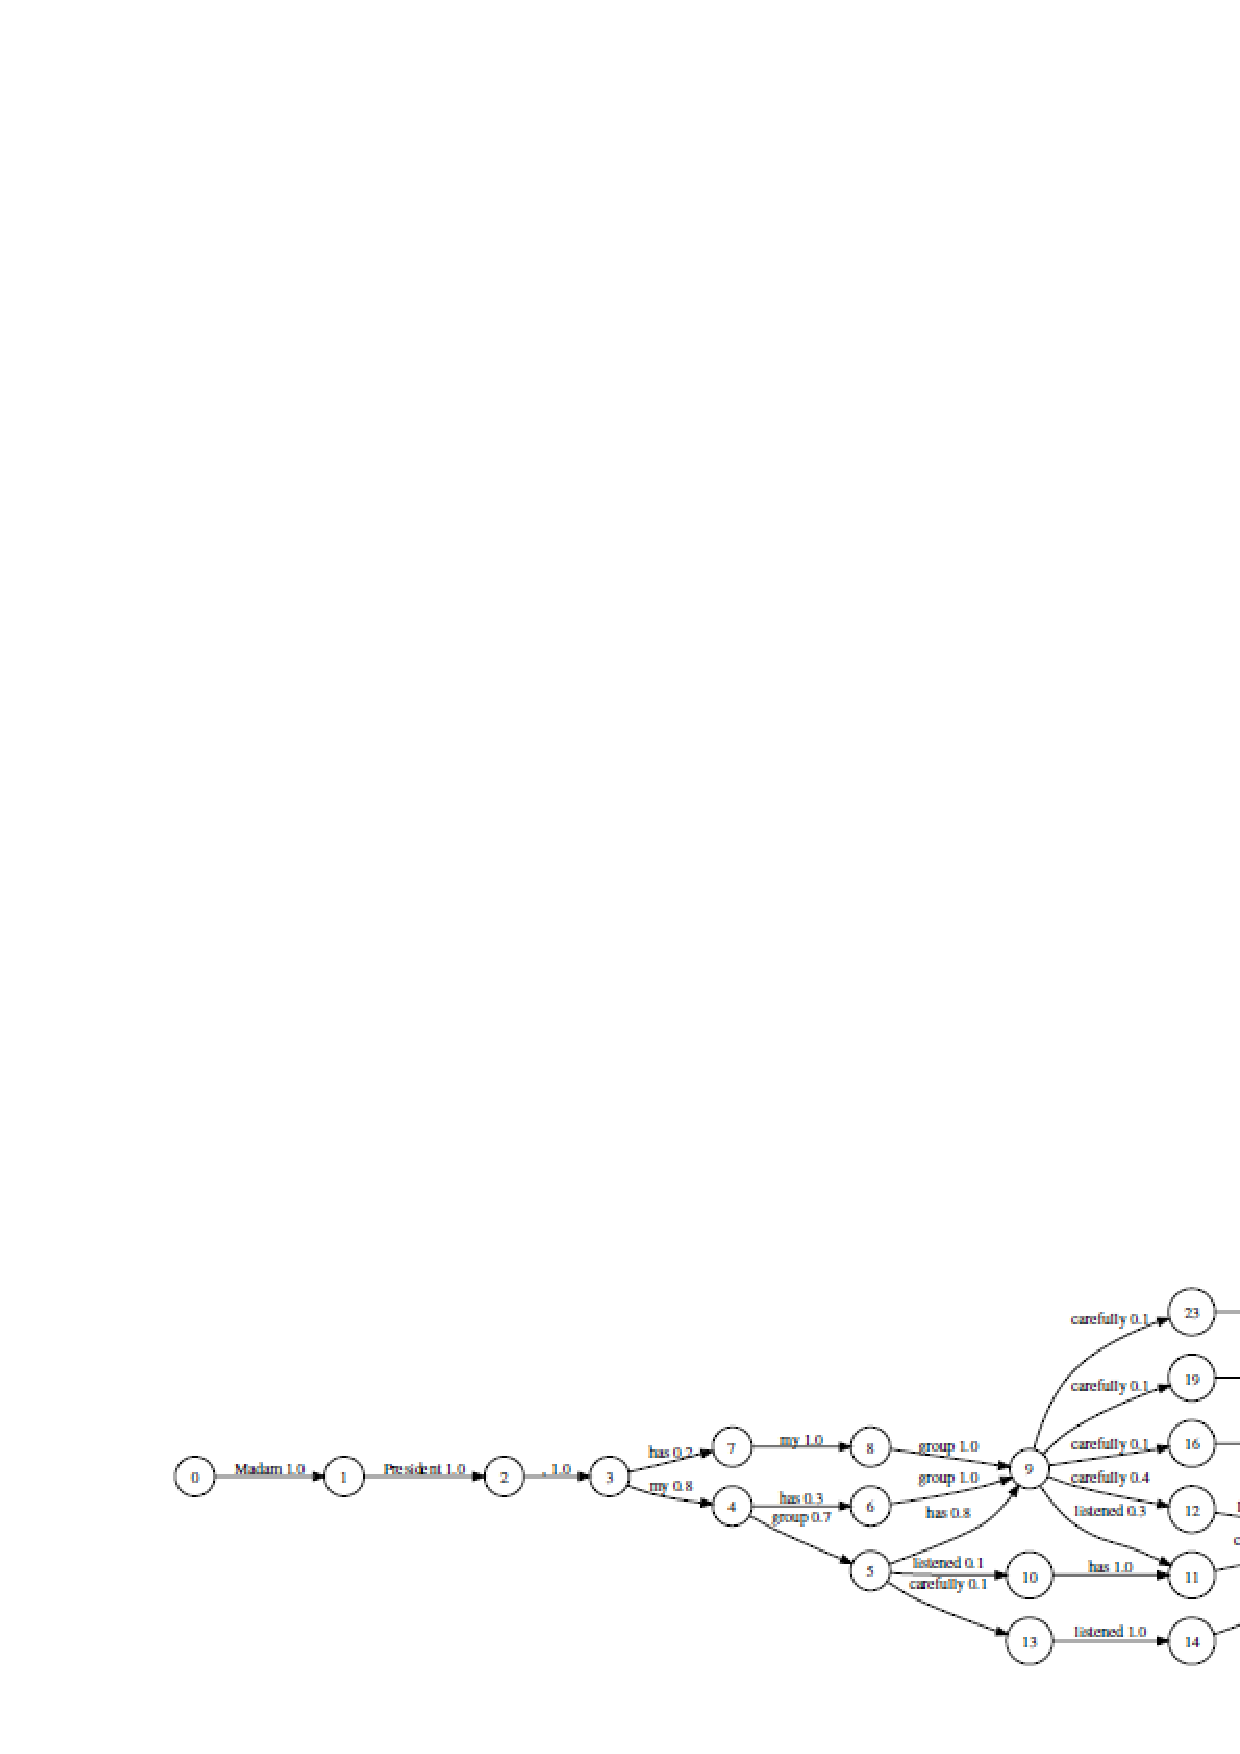
\includegraphics[scale=0.25]{lattices.png}
\end{figure}
\end{frame}


\begin{frame}{Rule Types}
\begin{itemize}
\item Short Rules\\
\hspace{2em}\textcolor{blue}{JJ NN} $\rightarrow$ 1 0 --- 0.573 \\
\item Long Rules\\
\hspace{2em}\textcolor{blue}{NN ADV * VAFIN} $\rightarrow$ 0 3 1 2 --- 0.18\\
\item Tree Rules\\
\hspace{2em}NP ( \textcolor{blue}{ADJP NNS} ) $\rightarrow$ 1 0  --- 0.103279\\
\item Multilayer Tree Rules\\
\hspace{2em}ADJP ( \textcolor{blue}{JJ} PP ( \textcolor{blue}{IN NP} ) ) $\rightarrow$ 0 2 1 --- 0.02988506\\
\end{itemize}
\end{frame}


\begin{frame}{Extracting Rules {\hfill \small \color{black} VP ( PTNEG NP VVPP ) $\rightarrow$ 0 2 1}}
\begin{figure}
\centering
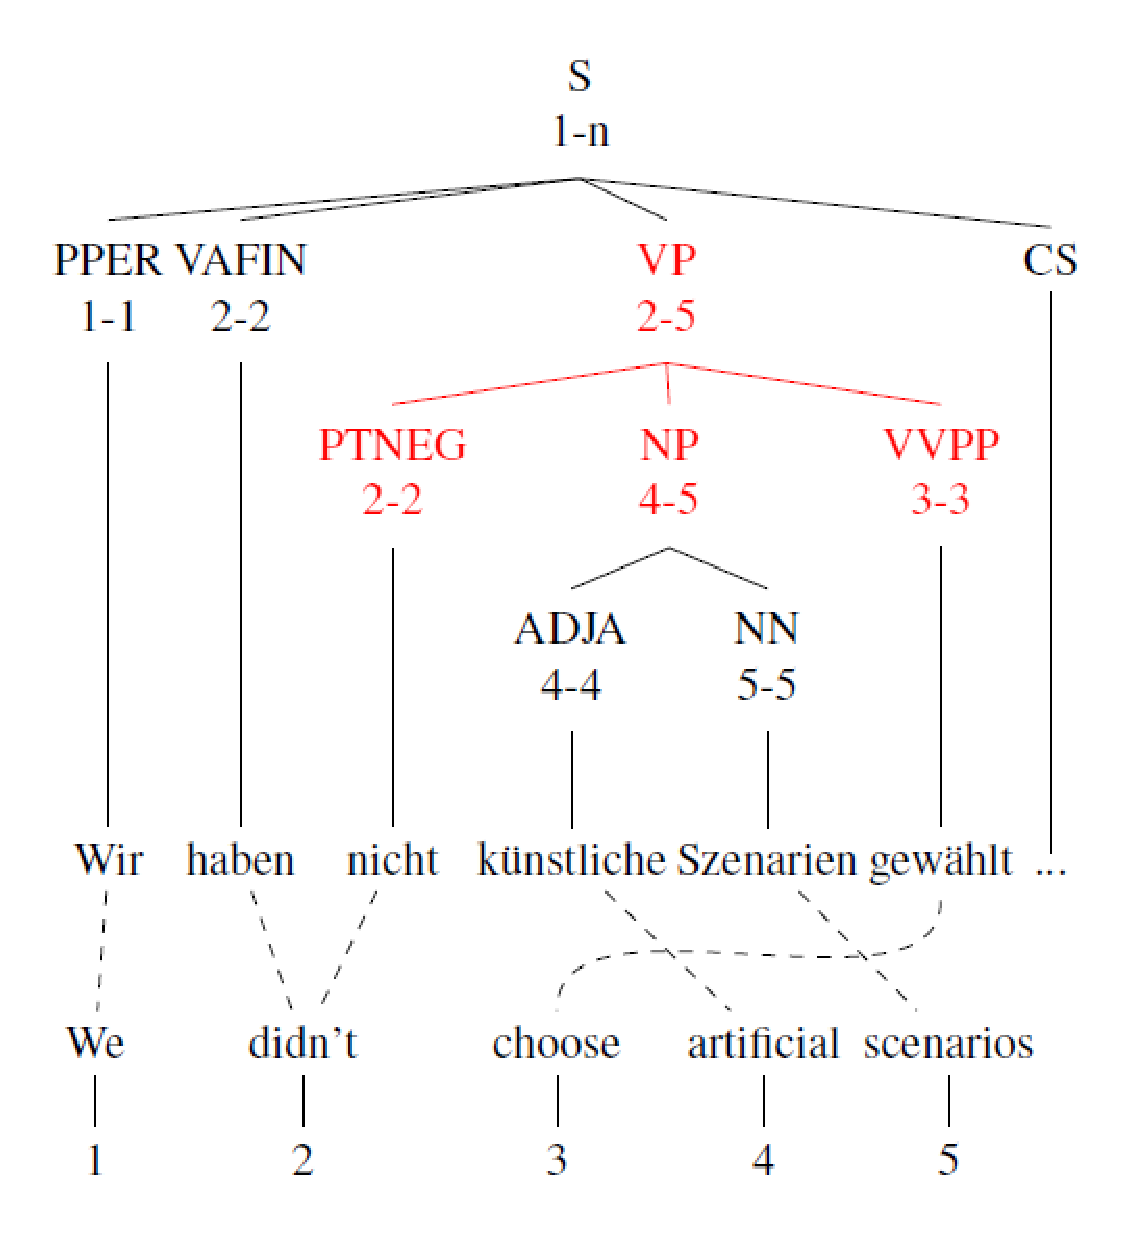
\includegraphics[scale=0.4]{extraction.eps}
\end{figure}
\end{frame}

\begin{frame}{Extracting Rules {\hfill \small \color{black} VP ( \textcolor{red}{PTNEG} NP ( \textcolor{red}{ADJA NN} ) \textcolor{red}{VVPP} ) $\rightarrow$ 0 3 1 2}}
\begin{figure}
\centering
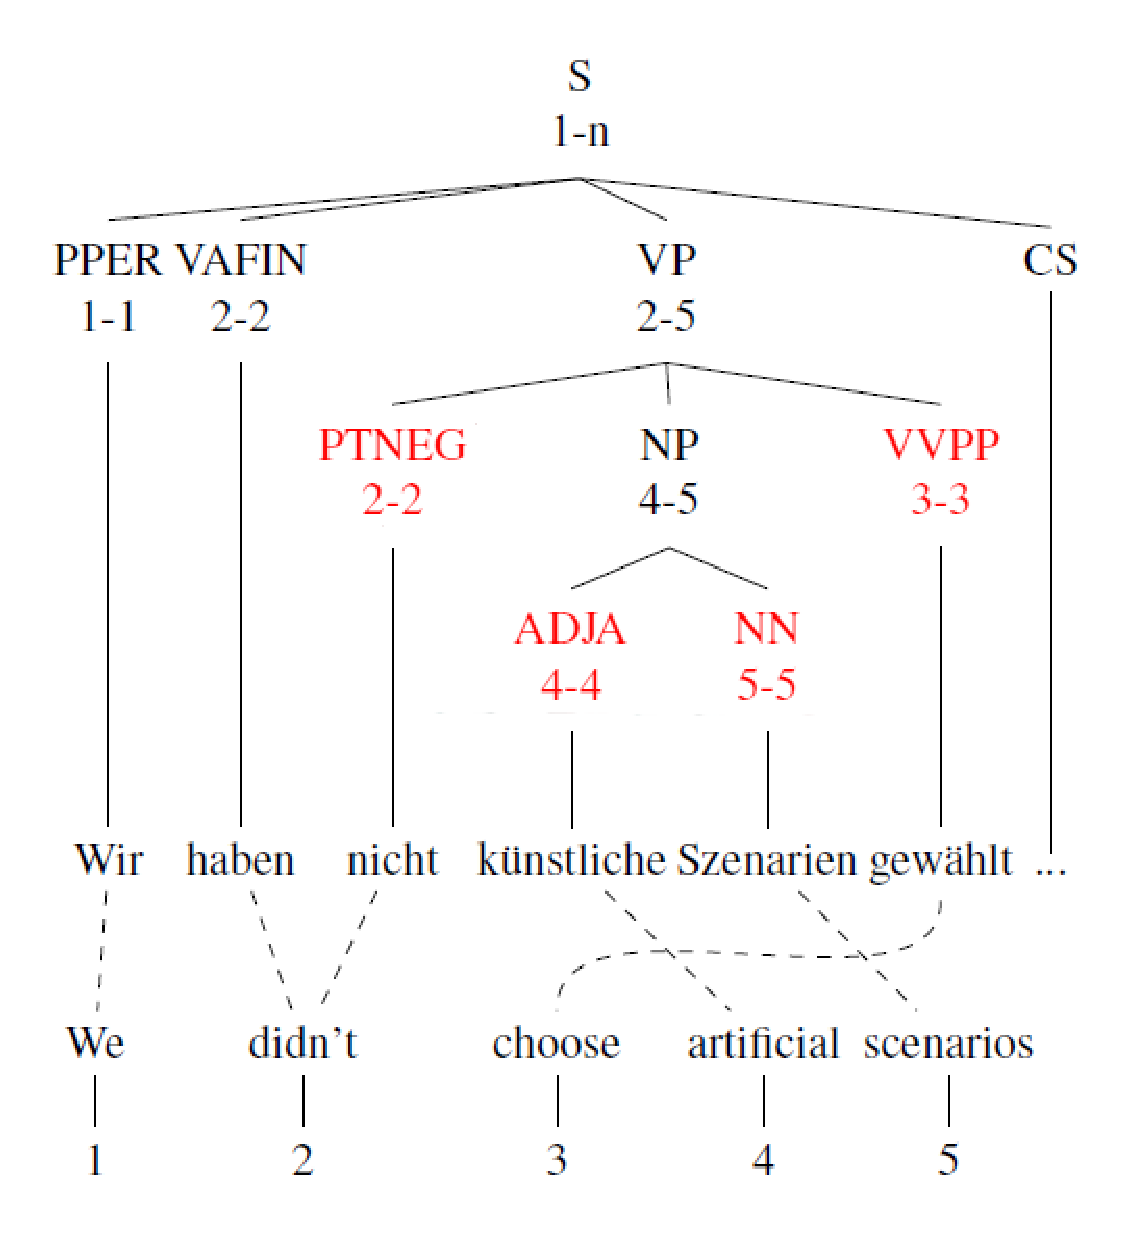
\includegraphics[scale=0.4]{extraction2.eps}
\end{figure}
\end{frame}

\begin{frame}{Evaluation}
\begin{tabular} {lll}
System & Rule \# & BLEU Score \\\hline
Baseline & & 8.09 \\
Short Rules & 95584 & 8.52 \\
Long Rules & 12306 & 8.57 \\
Tree Rules & 1573 & 8.79 \\
Combined & 109456 & 8.93 \\
Multilayer Tree Rules (layers = 2) & 4029 & 9.04 \\
\vspace{1cm}
\end{tabular}

Training Data: English $\rightarrow$ Chinese, 75873 lines, 12.4MB
\end{frame}

\begin{frame}[fragile]{Vector Representation as Feature}
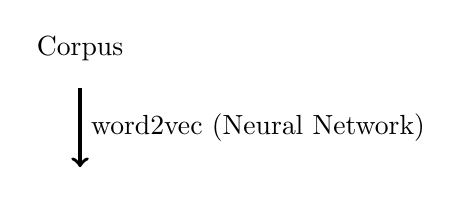
\begin{tikzpicture}
\tikzstyle{myarrows}=[->,line width=0.45mm];
\node[rectangle] at (0,0) {Corpus};
\draw[myarrows] (0,-0.5) -- node[auto] {word2vec (Neural Network)} (0,-1.5);
\end{tikzpicture}
\vspace{0.3cm}
\hrule
\begin{verbatim}
...
spain    -0.274035 -0.153813 -0.073527 -0.080498 ...
larger   -0.000062  0.030795 -0.152307 -0.286478 ...
products -0.348087 -0.112983  0.120410 -0.176838 ...
parties  -0.259261 -0.040402 -0.047077 -0.312133 ...
night     0.096195  0.019403  0.063992  0.248290 ...
...
\end{verbatim}
       
\end{frame}

\begin{frame}[fragile]{Vector Representation as Feature}
\begin{verbatim}
Enter word or sentence (EXIT to break): translation

                  Word       Cosine distance
------------------------------------------------------------------------
          translations       0.652776
                 bible       0.620422
            translated       0.591767
                  text       0.564570
            septuagint       0.559373
            dictionary       0.557046
               tyndale       0.546539
               vulgate       0.542804
            translator       0.542666
             apocrypha       0.537319
           translators       0.526699
                   ...       ...
\end{verbatim}
\end{frame}

\end{document}
